\documentclass[11pt,a4paper]{article}
\usepackage[margin=1in]{geometry}
\usepackage[T1]{fontenc}
\usepackage[utf8]{inputenc}
\usepackage{lmodern}
\usepackage{microtype}
\usepackage{amsmath,amssymb,booktabs,graphicx,xcolor}
\usepackage{hyperref}
\usepackage{enumitem}
\usepackage{caption}
\usepackage{float}
\usepackage{listings}
\hypersetup{colorlinks=true,linkcolor=blue,citecolor=blue,urlcolor=blue}
\graphicspath{{../pilot/run_corrected/}}
\setlist{itemsep=2pt,topsep=3pt}
\emergencystretch=3em

\title{\textbf{Methodological Progress Report}\
\large Artifact-Aware Stability of Fractal Features in Depth-Indexed Well Logs}
\author{Master's Thesis Project (MTP)\\Progress report for research supervision}
\date{16 September 2026}

\begin{document}
\maketitle
\begin{abstract}
This report documents the first corrected implementation and bounded validation stage of an MTP on fractal-feature stability in depth-indexed well logs. The primary research question is whether established fractal descriptors remain recoverable and stable under sampling, filtering, and preprocessing perturbations. A corrected synthetic generator was implemented using exact circulant embedding of the stationary fractional Gaussian noise (fGn) covariance, followed by cumulative summation to obtain fractional Brownian motion (fBm)-like levels. The implementation was tested against the target covariance for $H\in\{0.2,0.5,0.8\}$ and then applied to three deterministically selected contiguous gamma-ray (GR) intervals from the public FORCE 2020 dataset. The synthetic recovery checks passed the prespecified bounded gate, while the real-data robustness gate failed because the variogram- and spectral-based H estimates disagreed substantially. The result is therefore a scientifically useful \emph{no-go} for a stable single-H interpretation on these intervals, not a failure of the generator or of the broader MTP direction. The report explicitly separates synthetic known-answer validation from descriptive real-log sensitivity.
\end{abstract}

\section{Introduction}
The MTP began with a literature review of fractal and multifractal methods used for reservoir and well-log analysis. Classical self-affinity and fractal-dimension work motivates the use of scaling descriptors \cite{hardy_fractals,schepers1992,hough1989}, while prior well-log studies demonstrate the application context but do not remove the need for estimator and artifact validation \cite{li2001,li2003,rahimi2018,partovi2017}. The review identified a methodological gap: many studies report fractal or multifractal attributes without establishing their sensitivity to finite record length, sampling, filtering, missingness, or geological regime mixing. The selected primary direction is therefore not a new estimator, but an artifact-aware benchmark for established estimators.

The central question is:
\begin{quote}
Under controlled sampling and filtering perturbations, which established fractal features extracted from depth-indexed well logs are recoverable, stable, and interpretable over a declared physical scale range?
\end{quote}

The current stage has two purposes: (i) validate the synthetic signal generator and estimator conventions against known parameters, and (ii) determine whether a small, reproducible real-GR pilot supports a stable single-H interpretation.

\section{Related work and project progress}
The assigned literature was inventoried and reviewed within the approved scope. The reservoir-fractals book was read only through Chapter 4. Forty initial research ideas were generated, screened, and consolidated into five detailed plans. The recommended primary idea is the stability benchmark; surrogate-controlled genuine multifractality is retained as an ambitious extension but is not part of the present report.

The FORCE 2020 public dataset was downloaded and verified previously. The dataset audit covered 118 LAS wells and approximately 2.34 million rows, with a common declared sampling interval of approximately 0.152~m in the inspected data. The present bounded pilot uses only processed/cleaned FORCE data and does not treat it as raw logging-tool ground truth.

\section{Corrected fBm/fGn formulation}
Let $0<H<1$ and define the unit-scale stationary fGn covariance at integer lag $k$ as
\begin{equation}
C_H(k)=\frac{1}{2}\left[(k+1)^{2H}-2k^{2H}+|k-1|^{2H}\right].
\label{eq:fgncov}
\end{equation}
The generator constructs a circulant embedding of this covariance sequence, computes its real Fourier eigenvalues, and rejects the embedding if materially negative eigenvalues are found. A Gaussian vector is transformed using the square root of these eigenvalues to produce stationary fGn increments $G_i$. The fBm-like level process is then defined by
\begin{equation}
B_0=0, \qquad B_j=\sum_{i=0}^{j-1}G_i.
\label{eq:cumsum}
\end{equation}
This distinction is essential: fBm levels are nonstationary but have stationary increments, whereas fGn itself is stationary. The implementation verifies the exact identity $B_{j+1}-B_j=G_j$ for every generated record.

For the variogram diagnostic, the pilot fits the log--log slope of the Matheron semivariogram on fBm-like levels and reports $H_{\mathrm{var}}=\alpha/2$. For the spectral diagnostic, the pilot applies the spectrum to first differences of the levels and uses the low-frequency fGn relation $H_{\mathrm{spec}}=(1-m)/2$, where $m$ is the fitted log-power versus log-frequency slope. No H values are clipped into $[0,1]$.

\section{Methods}
\subsection{Synthetic known-answer experiment}
The corrected generator was evaluated at $H=0.2$, $0.5$, and $0.8$, with four fixed seeds (11, 22, 33, and 44) and 8192 increments per realization. The prespecified bounded synthetic gate required, separately for each H and estimator, absolute mean bias no greater than 0.12 and RMSE no greater than 0.18. The fit used lags/wavelengths from 20 to 160 samples, a Hann-window Welch periodogram with 2048-sample segments and 50\% overlap, and no post-hoc tuning.

\subsection{Real-log selection and perturbations}
The real pilot considered LAS files in deterministic sorted relative-path order. For each well, the GR curve was read together with the LAS NULL value and depth coordinate. Invalid GR values and depth discontinuities split the record; no interpolation or gap-spanning analysis was used. The longest eligible contiguous uniform block was selected, and the first 4097 points were retained. The first three eligible wells were analyzed.

Each selected interval had four variants: baseline, Gaussian smoothing with $\sigma=0.304$~m, and polyphase anti-aliased downsampling by factors two and four. Forty native points were trimmed at both ends to remove boundary influence. All variants used the same physical depth endpoints and the same physical lag range, approximately 3.04--24.32~m. The real robustness gate required every absolute change from baseline to be at most 0.10 for each estimator and baseline variogram--spectral H disagreement to be at most 0.15.

\subsection{Reproducibility and provenance}
The implementation is in \texttt{pilot/experiment.py}; tests are in \texttt{pilot/test\_pilot.py}. The exact prespecification is in \texttt{pilot/PRESPEC.md}. The executed outputs are stored in \texttt{pilot/run\_corrected/}, including JSON results, selected-well manifest, compressed arrays, figures, and a generated report. The selection manifest records source paths, SHA-256 hashes, selected row ranges, depth ranges, declared step, and maximum step error.

\section{Results}
\subsection{Software and mathematical verification}
The test suite completed with four passing tests. It verified covariance reconstruction from the circulant eigenvalues, the Brownian case at $H=0.5$, exact cumulative increment recovery, invalid-input handling, contiguous-block selection, physical-grid consistency, anti-alias suppression, and saved pilot artifacts.

\subsection{Synthetic recovery}
Table~\ref{tab:synthetic} reports the executed synthetic results. The synthetic gate passed for both estimators at all three tested H values. These results support the implementation's known-answer behavior under the declared finite-band protocol; they do not constitute a comprehensive estimator validation because only four realizations per H were used.

\begin{table}[H]
\centering
\caption{Synthetic recovery from the corrected fBm/fGn generator. Bias is estimated H minus known H.}
\label{tab:synthetic}
\begin{tabular}{@{}rrrrr@{}}
\toprule
Known $H$ & Estimator & Bias & RMSE & Gate \\
\midrule
0.2 & Variogram & -0.0135 & 0.0270 & Pass \\
0.2 & Spectral & -0.0143 & 0.0653 & Pass \\
0.5 & Variogram & -0.0199 & 0.0333 & Pass \\
0.5 & Spectral &  0.0051 & 0.0637 & Pass \\
0.8 & Variogram & -0.0285 & 0.0463 & Pass \\
0.8 & Spectral &  0.0068 & 0.0637 & Pass \\
\bottomrule
\end{tabular}
\end{table}

\begin{figure}[H]
\centering
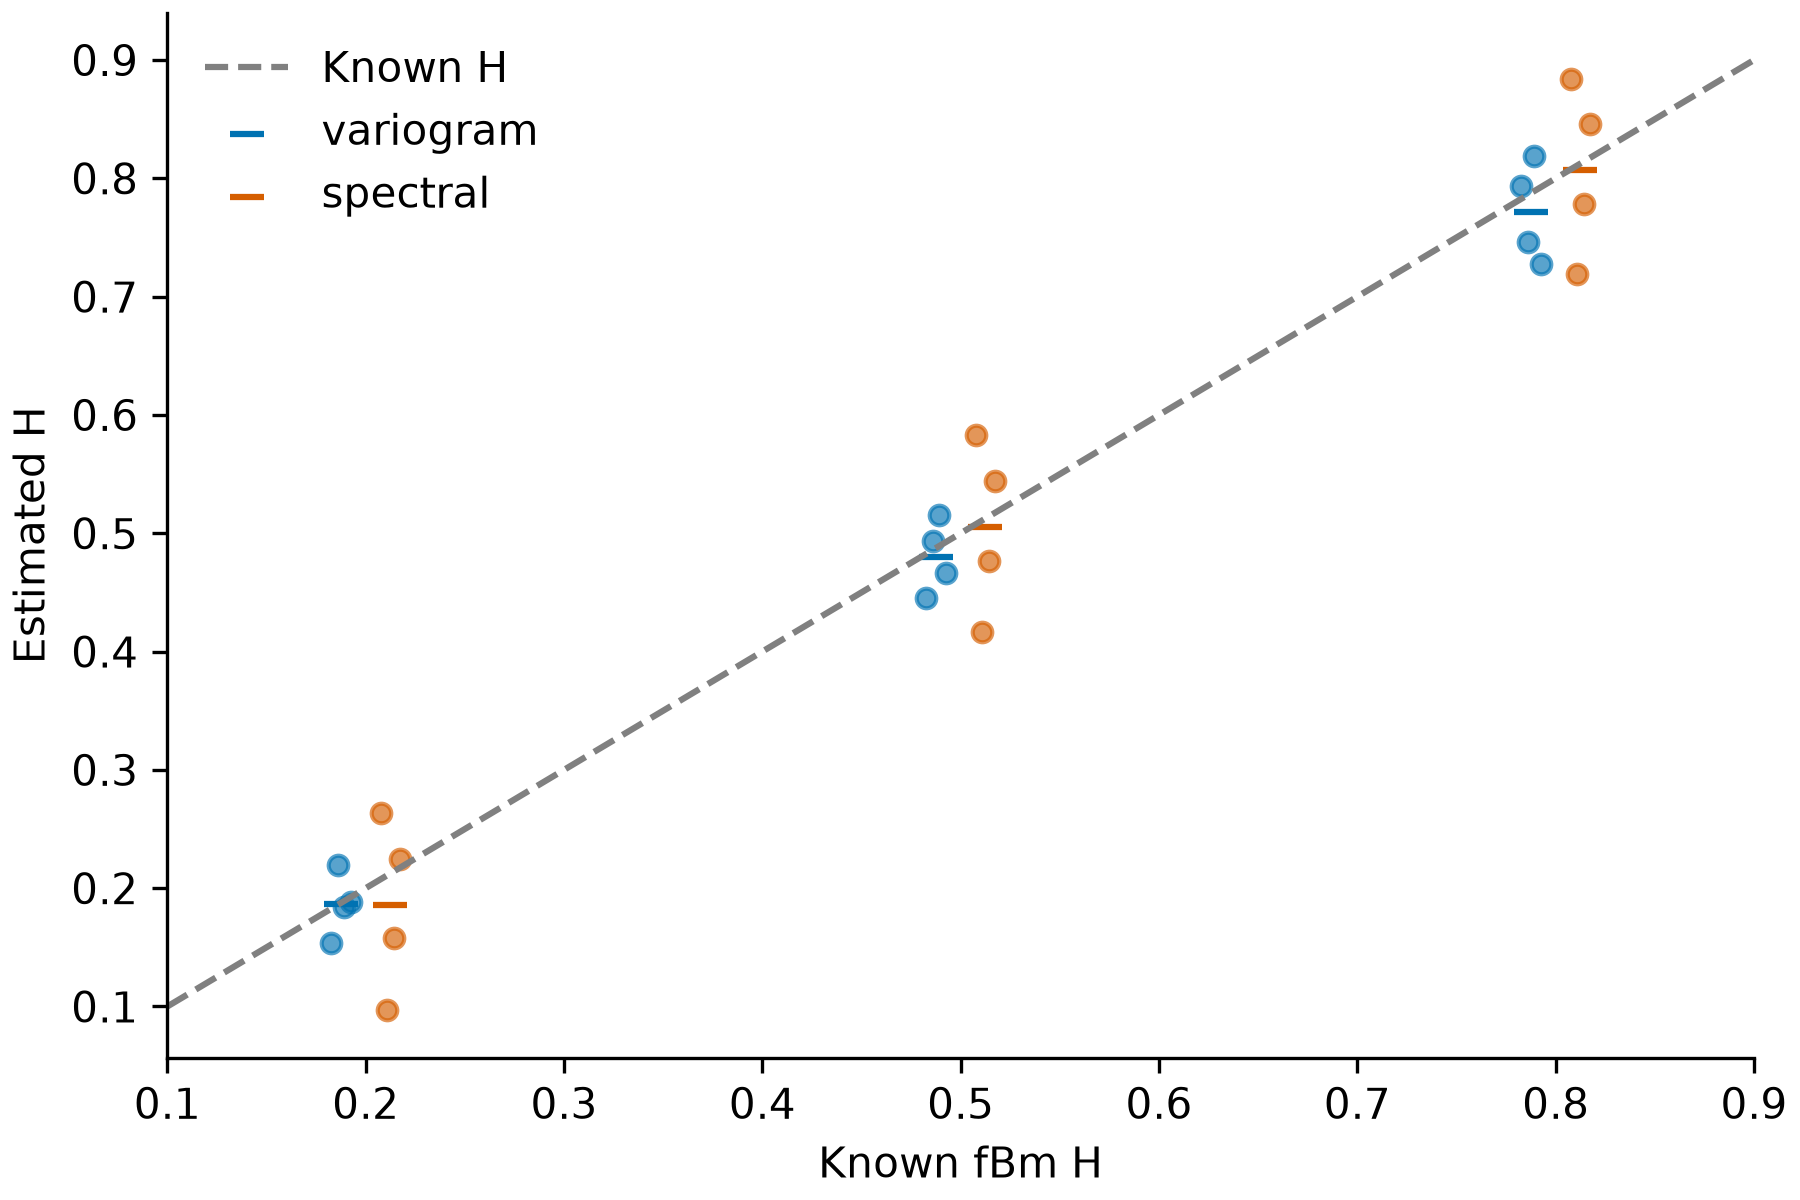
\includegraphics[width=0.94\textwidth]{Figure_1.png}
\caption{Synthetic estimates against known H values for the corrected generator. Individual seeds and estimator summaries are shown by the executed pilot plotting script.}
\label{fig:synthetic}
\end{figure}

\subsection{Real GR pilot}
The real robustness gate failed for all three selected intervals. The baseline estimates are shown in Table~\ref{tab:real}. The largest perturbation change remained below the 0.10 change threshold in the generated summary, but the baseline variogram--spectral disagreements were much larger than the 0.15 interpretation threshold. This means that the same real GR interval does not support one unqualified H value under the two diagnostics.

\begin{table}[H]
\centering
\caption{Real GR baseline summaries and largest absolute variant change.}
\label{tab:real}
\begin{tabular}{@{}lrrrr@{}}
\toprule
Well & Variogram H & Spectral H & Largest $|\Delta H|$ & Gate \\
\midrule
15\_9-13 & 0.3867 & -0.1087 & 0.0945 & Fail \\
15\_9-14 & 0.3382 &  0.1143 & 0.0944 & Fail \\
15\_9-15 & 0.3050 &  0.0163 & 0.0946 & Fail \\
\bottomrule
\end{tabular}
\end{table}

\begin{figure}[H]
\centering
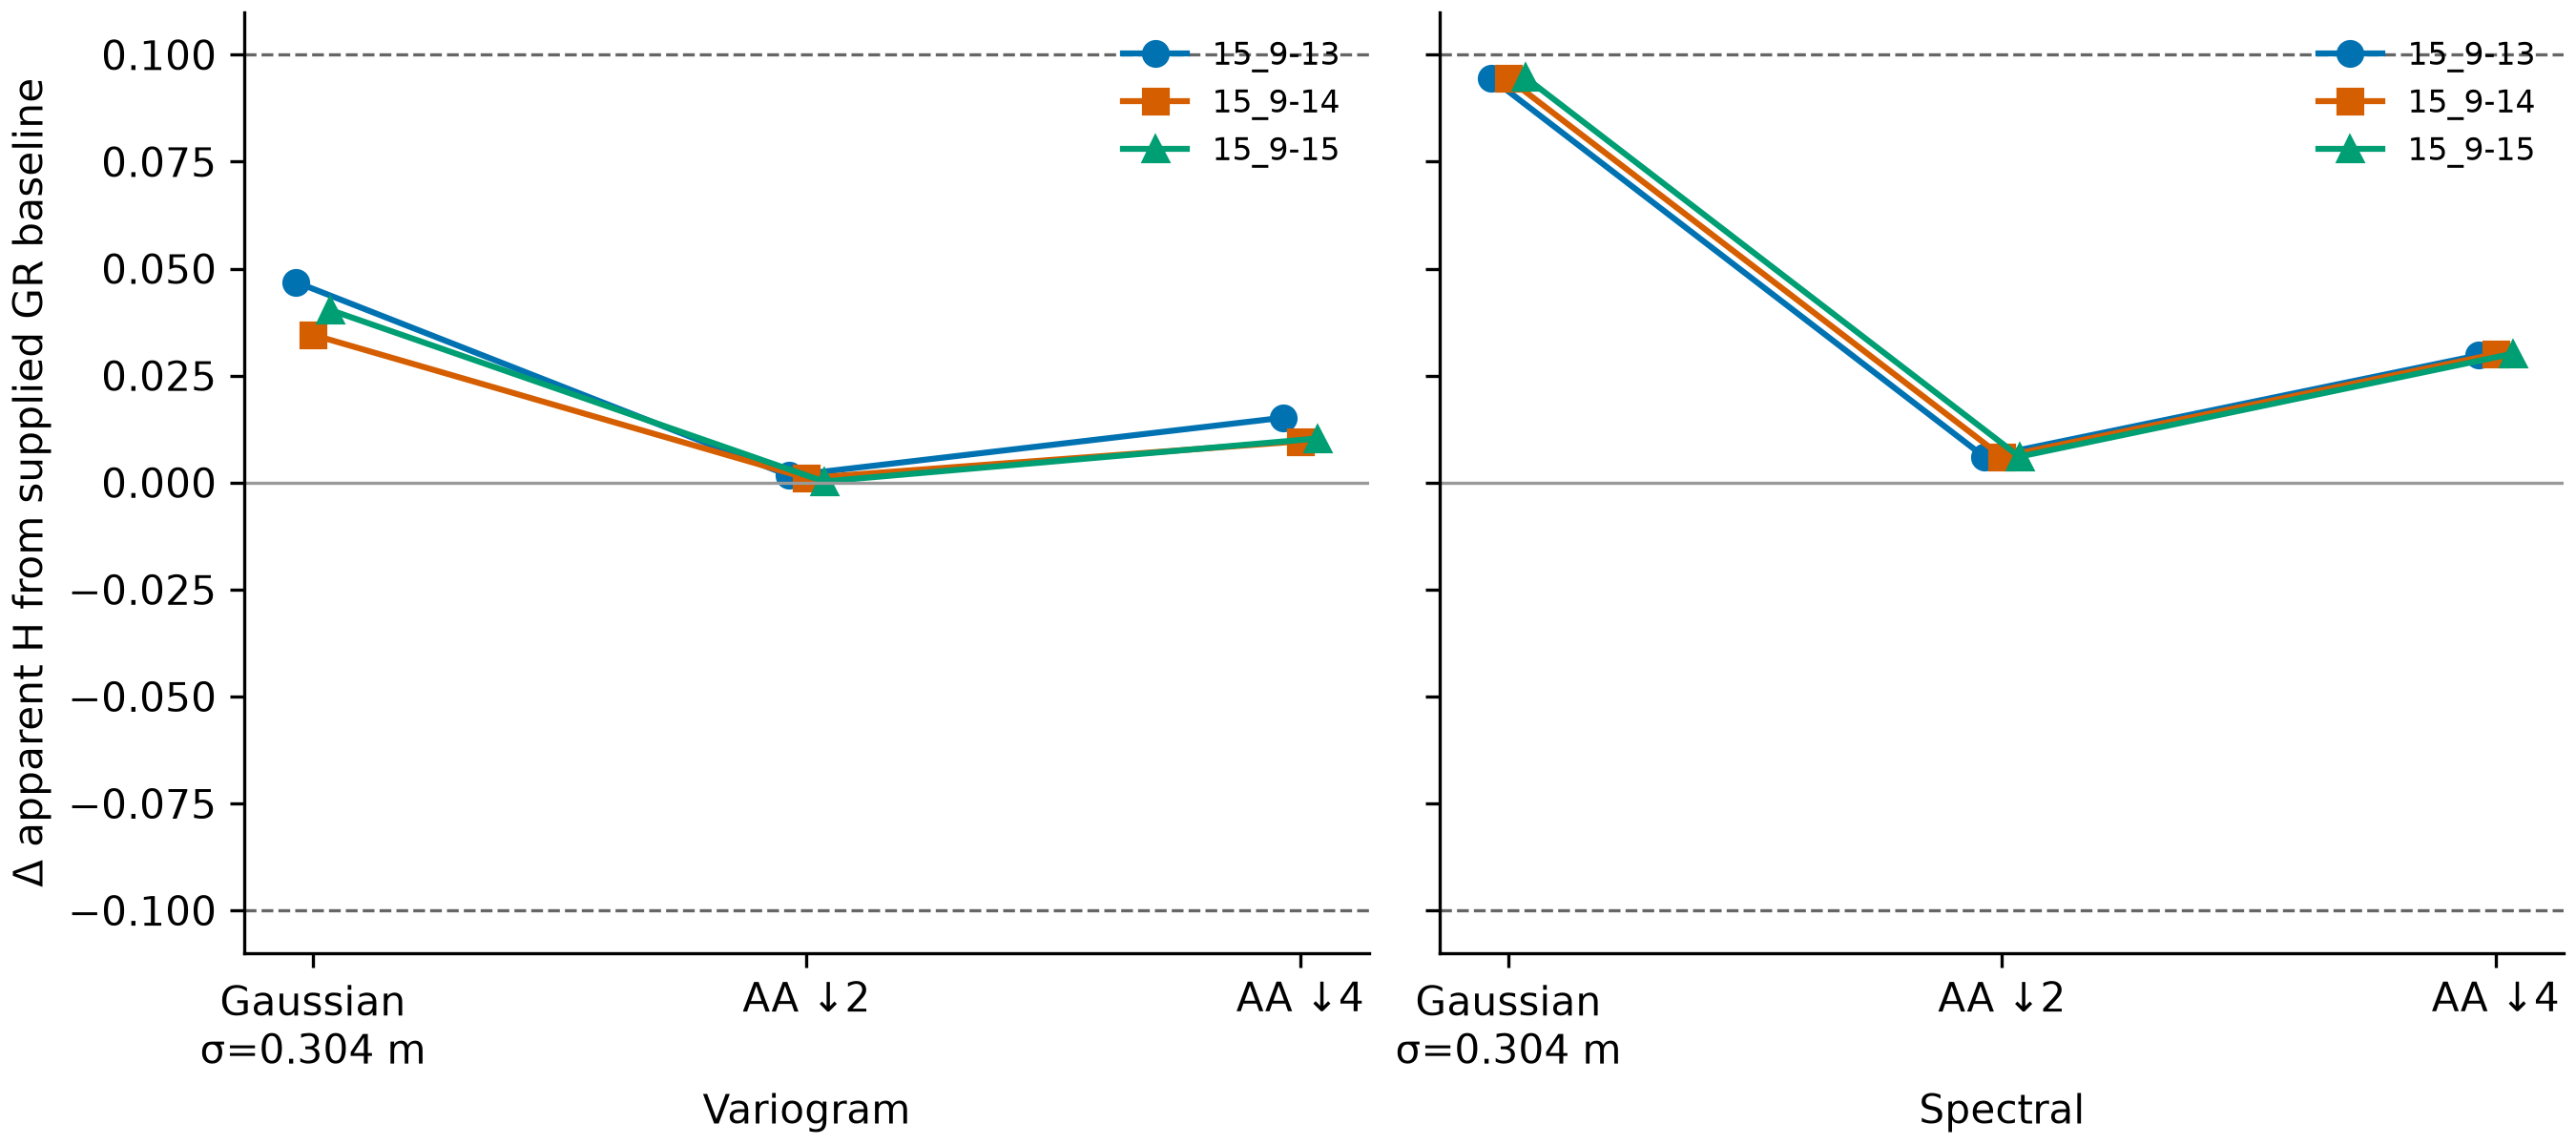
\includegraphics[width=0.94\textwidth]{Figure_2.png}
\caption{Change in real-log H estimates relative to each interval's baseline under smoothing and anti-aliased downsampling. The figure is descriptive and does not imply geological accuracy.}
\label{fig:real}
\end{figure}

\section{Interpretation}
The corrected implementation resolves the principal mathematical risk in the initial pilot: confusing a Fourier power-law control with a validated fBm/fGn process. The synthetic result demonstrates that the covariance-based generator and the declared estimator inputs are internally consistent over this bounded test. The real result provides the more important methodological warning: estimator agreement cannot be assumed merely because both diagnostics are called ``fractal'' measures.

The no-go decision applies narrowly to a stable single-H interpretation of the three selected GR intervals under the present protocol. It does not imply that the logs contain no scaling structure, nor that one estimator is universally superior. The observed disagreement may reflect finite-band effects, mixed geological regimes, trends, estimator-specific weighting of scales, and the fact that FORCE curves are processed rather than raw tool observations.

\section{Limitations}
\begin{enumerate}
\item The synthetic check used four seeds per H, whereas a formal Monte Carlo validation should use at least 30 independent evaluation realizations per H and report uncertainty of the aggregate metrics.
\item The real pilot used three intervals and therefore cannot support population-wide claims across wells or formations.
\item The Gaussian smoothing kernel is a controlled numerical perturbation, not a measured logging-tool transfer function.
\item The selected intervals were deterministic contiguous GR windows, not facies- or formation-homogeneous windows; geological regime mixing remains possible.
\item No lithology prediction, porosity/permeability prediction, graph dimension claim, or genuine multifractality claim is made.
\item The real logs are cleaned/despiked FORCE products and cannot provide independent raw-tool ground truth.
\end{enumerate}

\section{Next steps}
The immediate next stage is to expand the corrected synthetic calibration to at least 30 realizations per H, add explicit covariance and increment diagnostics, and freeze the physical passbands before evaluating estimator stability. The real-data protocol should then be extended to a predetermined set of contiguous windows with a rejection ledger and geological-context annotations. Only after the monofractal calibration and scale-quality gates are satisfactory should a measure-specific multifractal/surrogate experiment be considered.

\section{Conclusion}
The corrected fBm/fGn generator has been implemented and exercised successfully. It produces covariance-consistent fGn increments and cumulative fBm-like levels, and the automated test suite passes. The bounded synthetic recovery gate passes, while the real robustness gate returns a transparent no-go for a stable single-H interpretation on the three pilot intervals. This is an actionable MTP result: preprocessing and estimator choice materially affect reported fractal attributes, so the thesis should prioritize artifact-aware physical-scale validation before geological interpretation or multifractal expansion.

\appendix
\section{Artifact index}
\begin{itemize}
\item Source implementation: \url{/home/ancientai/Projects/serious/MTP/pilot/experiment.py}
\item Tests: \url{/home/ancientai/Projects/serious/MTP/pilot/test_pilot.py}
\item Prespecification: \url{/home/ancientai/Projects/serious/MTP/pilot/PRESPEC.md}
\item Executed result JSON: \url{/home/ancientai/Projects/serious/MTP/pilot/run_corrected/final_info.json}
\item Selection manifest: \url{/home/ancientai/Projects/serious/MTP/pilot/run_corrected/selection_manifest.json}
\item Generated pilot summary: \url{/home/ancientai/Projects/serious/MTP/pilot/run_corrected/report.md}
\end{itemize}

\bibliographystyle{plain}
\bibliography{references}
\end{document}
